\chapter{Johdanto}
Perinteisesti yritysten käyttämät toiminnanohjausjärjestelmät tai muut olennaiset ohjelmistot ovat olleet asennettuina asiakkaan omille laitteille. Ohjelmistojen alettua siirtyä enenevissä määrin pilviympäristöihin, myös palveluiden palvelinkustannusten optimointi on noussut olennaiseksi kysymykseksi. Kun ohjelmisto onkin ajossa pilvipalvelussa perinteisen oman palvelinympäristön sijaan, on mahdollista tehostaa palvelinten käyttöastetta moniasiakasmallia hyödyntämällä.

Moniasiakasjärjestelmää suunnitellessa on kuitenkin omat haasteensa, jotka voivat aiheuttaa suoria ja epäsuoria kustannuksia. Tämän tutkielman tarkoituksena on pureutua näihin kysymyksiin ja selvittää millaisia haasteita moniasiakaspalveluissa on aiemmin havaittu ja miten näitä on ratkaistu.

Moniasiakasjärjestelmät ovat nykyään huomattavasti yleistyneet. Niiden haasteiden tutkiminen on kuitenkin edelleen mielenkiintoista, jotta voidaan tunnistaa tilanteet, joihin tällainen malli ei sovellu tai millaisissa tapauksissa asiakaskohtainen malli voi olla lopulta parempi ratkaisu. Vaikka moniasiakasmallin ja asiakaskohtaisten järjestelmien välillä vaihtaminen on jälkikäteen mahdollista, voi huomattavilta ylimääräisiltä kehityskustannuksilta \cite{momm2011qualitative} välttyä pohtimalla moniasiakasmallin haasteita ja hyötyjä jo toteutusvaiheessa.

Tässä tutkielmassa moniasiakasjärjestelmien haasteita selvitetään tutkimalla tapauksia tällaisista järjestelmistä, joista on kirjoitettu riittävän laaja ja luotettava kuvaus. Lisäksi moniasiakasjärjestelmän määrittelemiseksi ja aiheen pohjustamiseksi on käytetty aiemmin aiheesta kirjoitettuja artikkeleita.

Ensimmäisessä kappaleessa määritellään moniasiakasjärjestelmä tämän tutkielman puitteissa, määrittämällä oleelliset piirteet, joissa se eroaa perinteisestä asiakaskohtaisesta järjestelmästä. Toisessa kappaleessa esitellään tutkitut moniasiakasjärjestelmän tapaukset. Kolmannessa kappaleessa tutkitaan eri toteutuksien eroja ja yhtäläisyyksiä, ja vedetään yhteen yleisimmät haasteet.

\chapter{Moniasiakasjärjestelmän oleellisia piirteitä}
Moniasiakasjärjestelmistä puhuttaessa voidaan viitata hyvinkin erilaisiin kokonaisuuksiin. Tässä luvussa määritellään moniasiakasjärjestelmä tämän tutkielman puitteissa ja tutkitaan, miten se poikkeaa asiakaskohtaisesta järjestelmästä. Bezmer ja Zaidman \cite{bezemer2010multi} määrittelevät moniasiakasjärjestelmän suoraviivaisesti ja selkeästi: Moniasiakasjärjestelmä sallii asiakkaiden jakaa sama laitteisto tarjoamalla käyttöön jaettu ohjelmiston ja tietokannan instanssi, samalla mahdollistaen ohjelman mukauttamisen asetuksilla omiin tarpeisiinsa.

Bezmer ja Zeidman on lisäksi nostanut esiin seuraavia oleellisia piirteitä moniasiakasjärjestelmistä:

\begin{enumerate}
  \item Järjestelmässä on asiakkaiden kesken jaetut fyysiset palvelimet.
  \item Järjestelmä on asiakaskohtaisesti muokattavissa käyttäjien tarpeiden mukaan.
  \item Järjestelmässä on asiakkaiden kesken jaetut tietokannat ja ohjelmiston ajossa olevat instanssit.
\end{enumerate}

\begin{figure}[h]
  \centering
  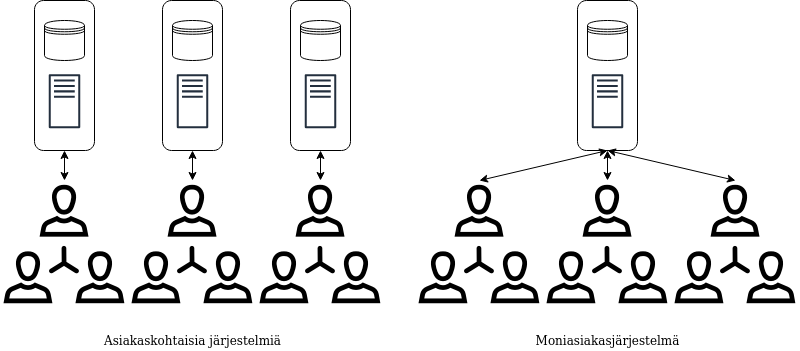
\includegraphics[width=16cm]{kuvat/yksi_vs_moni.png}
  \caption{Moniasiakasjärjestelmässä jokainen asiakasorganisaatio käyttää samoja järjestelmän instansseja.}
\end{figure}

Useimmat nykyaikaiset ohjelmistopalvelut täyttävät nämä piirteet jossain määrin. Määritelmän rajaamiseksi tässä tutkielmassa erottelemme vielä tavalliset monen käyttäjän palvelut moniasiakasjärjestelmistä olettamalla, että moniasiakasjärjestelmässä on useita organisaatioita, joista jokaisella voi olla useita käyttäjiä ja käyttäjäryhmiä.

\section{Jaetut palvelimet}
Kaikki asiakkaat käyttävät samaa fyysistä laitteistoa. Tämän avulla moniasiakasjärjestelmässä saavutetaan asiakaskohtaisia järjestelmiä parempi kustannustehokkuus. Kun kaikki asiakkaat jakavat saman laitteiston, saadaan käyttöaste paremmaksi. Tämä osaltaan aiheuttaa joitain haasteita, joita käsitellään myöhemmissä luvuissa.

Jaettuja palvelimia voidaan hyödyntää myös käyttämättä moniasiakasjärjestelmää, esim. ajamalla asiakaskohtaisia järjestelmiä virtualisoiduissa ympäristöissä. Tämä voi tapahtua joko asiakkaan omilla palvelimilla, tai pilvipalveluja hyödyntämällä. Näin voidaan saavuttaa merkittäviä hyötyjä asiakaskohtaisiin palvelimiin verrattuna, mutta virtualisoinnin aiheuttama resurssihukan takia hyötysuhdetta ei saada yhtä hyväksi kuin jaetuilla instansseilla.

\section{Jaetut tietokannat ja ohjelmiston ajossa olevat instanssit}
Jaetun fyysisen laitteiston lisäksi palvelimia ei ole jaettu asiakkaiden kesken esimerkiksi erillisillä virtualisoiduilla ympäristöillä. Virtualisoituihin ympäristöihin verrattuna tässä arkkitehtuurissa on etuna se, että se ei aiheuta samanlaista resurssihukkaa, kuin kokonaisten ympäristöjen virtualisointi \cite{huber2011evaluating}.

Erityisesti asiakkaiden kesken jaetut tietokannat vaativat ohjelmiston suunnittelun kannalta erityistä huomiota. Koska asiakkaiden data sijaitsee samassa tietokannassa ja samoissa tauluissa, täytyy tietojen näkyvyys asiakkaiden välillä ratkaista ohjelmiston tasolla.

Tietokannan jakaminen asiakkaiden välillä voidaan toteuttaa joko siten, että samassa tietokannassa on asiakaskohtaiset taulut, tai jakamalla tiedot rivikohtaisesti asiakkaiden välillä. Asiakaskohtaiset taulut ovat helppo tapa eriyttää data ja toteuttaa pääsynhallinta asiakkaiden tietojen välillä. Samalla tietokannan taulujen määrä kasvaa huomattavasti, joka aiheuttaa sen, ettei yhdellä tietokannalla voi palvella yhtä monta asiakasta kuin käyttämällä jaettuja tauluja \cite{chong2006multi}.

\section{Palvelun asiakaskohtainen muokattavuus}
Palvelun asiakaskohtainen muokattavuus on usein olennainen piirre moniasiakasjärjestelmässä, koska sillä on tarkoitus korvata asiakaskohtaiset asennukset, joissa tyypillisesti on tehty erilaisia räätälöintejä kullekin asiakkaalle. Koska kaikki asiakkaat käyttävät samaa instanssia ohjelmistosta, ei ohjelmakoodia muokkaamalla voida tehdä asiakaskohtaisia muutoksia. Ohjelmakoodissa täytyy siis jo suunnitteluvaiheessa ottaa huomioon riittävä sovelluksen muokattavuus, ja asiakkaiden täytyy voida muuttaa ohjelman toimintaa ajonaikaisesti.

Ohjelmiston muokattavuuden tarpeet voivat olla hyvin eritasoisia. Yksinkertaisimmillaan järjestelmässä riittää pienet ulkoasun muokkaukset, mutta monimutkaisissa tapauksissa käyttäjät voivat luoda täysin omiin tarpeisiinsa erilaisia tietomalleja. Useimmiten tarve on jotain tältä väliltä, esimerkiksi omien työvaiheiden määrittämistä toiminnanohjausjärjestelmässä.

\chapter{Tapauksia moniasiakasjärjestelmistä}
Moniasiakasjärjestelmistä yleisesti on kirjoitettu jonkin verran, mutta hyvin raportoituja toteutuksia on niukasti saatavilla. Tässä luvussa käsittelen löytämiäni riittävän hyvin kuvattuja järjestelmiä ja pyrin tiivistämään järjestelmän arkkitehtuurin kannalta olennaiset ratkaisut ja ongelmat joita niillä on ratkaistu. Tapauksiksi on valittu Force.com \cite{weissman2009design}, IBM:n sähköisten sopimusten hallintajärjestelmä \cite{kwok2008software} ja ScrewTurn Wikin muunnos moniasiakasjärejestelmäksi \cite{bezemer2010challenges}.


\section{Force.com}
Force.com on SalesForce-yrityksen alusta, jota yli 50 000 organisaatiota käyttää oman ohjelmistopalvelunsa kehittämiseen. Alusta on moniasiakasjärjestelmäksi rakennettu, eli kaikki asiakkaat jakavat saman alusta, ilman erillisiä asiakaskohtaisia laitteistoja, tietokantoja tai muita ohjelmistoja. Weissman ja Bobrowski ovat kirjoittaneet kattavan kuvauksen \cite{weissman2009design} järjestelmän toteutuksesta.

Force.comin arkkitehtuuri on poikkeava normaalin ohjelmistopalvelun tavanomaisesta arkkitehtuurista, koska se on alusta, jossa samaan jaettuun järjestelmään voidaan rakentaa useita täysin erityyppisiä palveluja. Tämän takia alusta määrittelee kaiken metatietojen avulla. Esimerkiksi käyttäjän luodessa uusi taulu palveluunsa, järjestelmä luo tämän uuden taulun kuvauksen metatietona, jolla mallinnetaan halutunlainen virtuaalinen tietokantataulu kaikkien jakamaan hyvin geneeriseen tietokantamalliin. Virtuaalinen tietokantataulu tulkitaan ajonaikaisesti ja siihen tehdyt tietokantakyselyt muutetaan muotoon, jolla tiedot voidaan hakea hyvin joustavasti muotoillusta asiakkaiden kesken jaetusta tietokannasta.

Tällaisen erittäin joustavan tietokantarakenteen takia tavanomaisten tietokantaindeksien tekeminen kyselyjen optimoimiseksi ei ole mahdollista. Koska Force.comin tietokantataulun sarakkeet eivät ole kiinteästi tyypitetty, joudutaan asia ratkaisemaan toisin. Tätä varten järjestelmässä on oma taulu indekseille, jossa tieto on tyypitettynä ja se on indeksoitu. Tätä taulua hyödynnetään tietokantakyselyjen optimoimiseksi, kun käyttäjä hakee dataa tietokannasta. Lisäksi tietokantahakujen tehostamiseksi data on osioitu kannassa asiakastunnisteen perusteella.



\section{IBM:n sähköisten sopimusten hallintajärjestelmä}
Kwok ym. \cite{kwok2008software} kuvailevat IBM:n tutkimusryhmän kokeilua toteuttaa sähköisten sopimusten hallinnointijärjestelmä moniasiakasjärjestelmänä suunnitelluksi palveluksi. Raportin kirjoituksen aikaan 2008 palvelua oli pilotoitu yli 10 organisaatiolle ja yli 300 käyttäjälle, jotka kaikki jakavat samat resurssit. Tutkimusryhmän mukaan vastaava palvelut on perinteisesti toteutettu asiakaskohtaisina järjestelminä, joiden kustannukset tällaisina ovat niin suuret, ettei pienillä yrityksillä ole niihin varaa.

Ohjelmistossa on toteutettu erillinen autentikaatiopalvelu (Security services), joka merkitsee kunkin sisäänkirjautuneen käyttäjän asiakaskohtaisella tunnisteella. Tältä palvelulta ohjelmiston muut moduulit hakevat käyttäjälle tunnisteen, jonka perusteella palvelu mukautetaan ja näytettävät tiedot valitaan. Asiakaskohtaisia ohjelmiston mukautuksia hallitaan ja säädetään ohjelmiston metatietopalvelussa (Metadata services). Näillä molemmilla palveluilla on omat erilliset tietokannat (käyttäjätietojen tietokanta ja asiakkaan metatietojen tietokanta).

Käyttäjien sisäänkirjautuminen on järjestelmässä toteutettu keskitetyn autentikointipalvelun avulla. Tämä ratkaisu on helppo toteuttaa, koska se ei vaadi mitään asiakaskohtaista osuutta, mutta samasta syystä integraatio asiakkaan jo olemassa oleviin järjestelmiin on haasteellinen, eikä sitä ole tässä järjestelmässä toteutettukaan. Käyttäjä siis joutuu aina erikseen kirjautumaan tähän palveluun, eikä saumatonta kokemusta asiakkaan muiden järjestelmien välillä voida saavuttaa.

Käyttäjäkohtaista muokattavuutta varten järjestelmän tietokantamalliin on suunniteltu rakenne, johon voidaan tehdä joustavasti lisäyksiä määrittäen tarvittaville lisätiedoille tietokannassa oma rivikohtainen tyyppi ja tunniste. Mukautettava rakenne monimutkaistaa tietokantakyselyjä ja tekee niiden tehostamisen indeksien avulla haastavammaksi.

Järjestelmässä on toteutettu erillinen moduuli asiakkaiden käytön seurantaan. Tämän avulla määritellään, kuinka paljon asiakkaita laskutetaan, mutta myös varmistetaan, että ohjelmiston tehokkuus pysyy vaaditulla tasolla. Raportissa ei ole käsitellä juurikaan järjestelmän tehokkuuden optimointia tai skaalausratkaisuja. Toisaalta raportin aikaan palvelun käyttäjämäärät ovat vielä olleet maltillisia, eikä skaalaus ole välttämättä ole ollut tarpeellista.

\section{ScrewTurn Wiki}
ScrewTurn Wiki on avoimen lähdekoodin ohjelmisto, jonka muuntamisesta moniasiakasjärjestelmäksi on tehty raportti osana tutkimusta \cite{bezemer2010challenges}. Raportissa on käsitelty tarvittavat muutokset autentikaatioon ja tietokantaan, sekä moniasiakasjärjestelmänä palvelun mukautettavuuden toteutus.

Käyttäjien tunnistaminen tapahtuu erillisellä Kerberos-protokollaa hyödyntävällä palvelulla. Tältä palvelulta saatavassa tunnisteessa voidaan tallentaa kaikki tarvittava tieto, jolla käyttäjän asiakkuus voidaan varmistaa. Lisäksi järjestelmässä on autentikaatiomoduuli, joka jokaisen palveluun tehtävän kyselyn yhteydessä tunnistaa käyttäjän asiakkuuden.

Järjestelmän muokattavuutta ei tässä tapauksessa toteutettu kattavasti. Joidenkin asetusten käsitteleminen integroitiin alkuperäisestä toteutuksesta käyttämään tätä varten kehitettyjä kirjastoja, jotka vastaavat palvelun mukautuksesta. Myös tietokanta on muunnettu moniasiakkuusmallia tukevaksi hyvin minimaalisin muutoksin. Tietokantaa varten on toteutettu abstraktiotaso, joka muuntaa kaikki tietokantakyselyt suodattamaan tulokset tunnistautumispalvelun antaman asiakastunnisteen perusteella.



\chapter{Johtopäätökset}

Tässä kappaleessa vertaillaan tutkittaviksi valittuja moniasiakasjärjestelmätoteutuksia. Olennaisiksi seikoiksi asiakaskohtaisiin ohjelmistoihin verrattuna valitsin tehokkuus, skaalaus, tietoturva ja ohjelmakoodin monimutkaistuminen. 

\section{Tehokkuus}
Koska jokaisen asiakkaan käyttäjät käyttävät ohjelmiston samaa instanssia, vaikuttaa heidän toimintansa järjestelmässä toisiinsa. Yhden asiakkaan aiheuttaessa ongelmatilanteen järjestelmään, voivat kaikkien asiakkaiden järjestelmät olla poissa käytöstä. Tästä syystä on erityisen oleellista, että käyttäjä ei pysty tekemään sellaista toimenpidettä järjestelmässä, jonka tehokkuus on niin huono, että se vaikuttaa muiden asiakkaiden käyttökokemukseen.

Moniasiakasjärjestelmien tehokkuudessa on oleellista panostaa tietokantakyselyiden tehokkuuteen, kun asiakasmäärät kasvavat suuremmiksi. Koska kaikkien asiakkaiden tiedot sijaitsee samoissa tietokantatauluissa, täytyy tietojen indeksointi tehdä järkevästi. Asiakastunnisteelle tehdään kaikissa tauluissa indeksit siten, ettei tietokantahakujen tehokkuus kärsi vaikka datamäärä on huomattavan suuri asiakaskohtaiseen tietokantaan verrattuna. Lisäksi tietokantahakuja voidaan optimoida tietokannan osioinnilla asiakkuustunnisteen perusteella, kuten Force.com palvelussa \cite{weissman2009design}. Toisaalta järjestelmän käytön monitoroinnin näkymä voi olla tehokkuuden tarkkailua varten hyödyllinen, kuten IBM:n tutkimusryhmä \cite{kwok2008software} kertoo.

Force.com ja IBM:n järjestelmän tehokkuuden optimoinnissa olennainen osa on tietokantakyselyiden optimointi moniasiakasmallia tukevalla tavalla. ScrewTurn Wikin kohdalla tehokkuutta varten ei toisaalta tehty vielä minkäänlaisia toimenpiteitä, luultavasti koska sitä ei ole testattu vielä raportin aikana suuremmilla käyttäjämäärillä.

\section{Skaalaus}
Moniasiakasjärjestelmän skaalaus on teknisesti asiakaskohtaisia asennuksia yksinkertaisempaa, koska järjestelmästä on vain yksi asennus, eikä skaalausta tarvitse tehdä jokaisen asiakkaan kohdalla erikseen. Toisaalta koska moniasiakasjärjestelmässä käyttäjien määrä moninkertaistuu asiakaskohtaiseen asennukseen verrattuna, ajaudutaan nopeammin tilanteeseen, jossa pelkkä palvelimen tehon lisäys ei enää riitä, vaan joudutaan ajamaan ohjelmistoa usealla palvelimella, joiden välillä kuormaa jaetaan.

IBM:n tutkimusryhmä \cite{kwok2008software} kertoo suunnittelevansa skaalauksen tarkempaa tutkimista vaihtamalla ohjelmisto tehokkaammille palvelimille, ajamalla ohjelmistosta useampaa instanssia samanaikaisesti, ja tehostamalla tietokannan toimintaa jakamalla se pienempiin segmentteihin. Force.comin tärkeäksi pullonkaulaksi mainitaan \cite{weissman2009design} metadatan lukeminen ohjelmistossa, koska kaikki asiakaskohtainen muokattavuus toteutetaan näiden avulla. Jotta järjestelmä skaalautuisi, metadatoja säilötään muistissa pidettävään välimuistiin. Bezmer ja Zaidman \cite{bezemer2010challenges} mainitsevat oman lähtökohtansa huomioivan skaalauksen siten, että kaikki ohjelmiston komponentit on toteutettu erillisinä irrallaan skaalattavina palveluina.

\section{Tietoturva}
Asiakaskohtaisessa asennuksessa voidaan tehdä erilaisia toimenpiteitä tietoturvan parantamiseksi, jotka moniasiakasjärjestelmässä ei ole mahdollista. Asiakaskohtaista järjestelmää voidaan esimerkiksi ajaa kokonaan asiakkaan omassa lähiverkossa, ilman että se on lainkaan yhteydessä julkiseen internetiin. Vaikka järjestelmä olisi julkisessa internetissä, sinne pääsy voidaan rajata eri tavoin vain kyseiselle asiakkaalle.

Moniasiakasjärjestelmässä kehittäjät joutuvat myös huolehtimaan, että asiakkaalla on pääsy vain omaan dataansa, koska kaikkien asiakkaiden data on sijoitettu samaan tietokantaan. Yleisesti tämä ongelma ratkaistaan siten, että asiakaskohtainen pääsynhallinta on sisäänrakennettu sovellukseen riittävän vahvasti. Kaikella tiedolla tietokannassa on siis asiakkaan tunniste, ja ohjelmistossa ei tietokantakyselyjä ei voi tehdä, ilman että kaikkiin kyselyihin on liitetty asiakkaan tunniste sisäänkirjautuneen käyttäjän perusteella.

Tietoturvan kannalta kaikissa tutkituissa tapauksissa on pääpiirteittäin samanlainen ratkaisu. Käyttäjien pääsynhallintaan ja tunnistautumiseen on erillinen palvelu, joka määrittelee käyttäjälle asiakkuustunnisteen. Tämä asiakkuustunniste liitetään järjestelmässä kaikkiin toimenpiteisiin, joita käyttäjä tekee, ja tietokantakyselyihin on toteutettu riittävä abstraktio, jolla kyselyitä ei ole mahdollista tehdä ilman asiakastunnistetta.

Tietoturvakompromissi joka moniasiakasympäristöissä ei ole ratkaistavissa kuten asiakaskohtaisessa kohtaisissa järjestelmissä, on kohdistetun hyökkäyksen mahdollisuus vaarantaa kaikkien asiakkaiden data kerralla. Toisin sanoen, jos hyökkääjä tahtoo päästä tietyn asiakkaan tietoihin käsiksi, onnistuessaan hän saa samalla kaikkien asiakkaiden tiedot. Tämän estämiseksi on asiakkailla väistämättä oltava vähintäänkin omat asiakaskohtaiset tietokannat.

\section{Ohjelmakoodin monimutkaistuminen}
Koska moniasiakasjärjestelmässä monia asioita, jotka ennen pystyttiin huomioimaan muilla tavoin, joudutaan nyt tekemään ajonaikaisesti ohjelmakoodissa, on se kehittäjille väistämättä monimutkaisempi. Tämän takia vaikka palvelinten ylläpidon puolelta työmäärä yksinkertaistuu ja vähenee, kehitystiimillä työtä on enemmän ja se on haastavampaa.

Eniten monimutkaisuutta aiheuttava tekijä moniasiakasjärjestelmissä on asiakaskohtainen muokattavuus. Koska tutkituissa tapauksissa asiakaskohtainen muokattavuus on toteutettu hyvin eri määrin, myös ohjelmakoodin ja järjestelmän arkkitehtuurin monimutkaisuus on tapausten välillä hyvin eritasoista.

Koska Force.com on alusta, jolle voi rakentaa hyvin vapaasti omanlaisensa ohjelmistopalvelun, on sen toiminnallisuus täysin käyttäjän määriteltävissä. Tämän takia myös ohjelmistossa on paljon monimutkaisia osia. Muihin järjestelmiin verrattaessa mielenkiintoista on tietokannan rakenne, joka sallii käyttäjän määritellä minkälaisen tahansa tietokantamallin. Tämä vaatii järjestelmältä paljon abstraktiota ja optimointia tietokannan päälle.

IBM:n digitaalisten sopimusten hallintajärjestelmässä käyttäjä pystyy tekemään erilaisia polkuja sopimusten hallinnointiin, ja lisäämään tietokantaan asiakaskohtaisia tietoja. Myös IBM:n järjestelmässä on tietokantaan siis toteutettu joustava osa, jolla asiakas voi lisätä omia tietorakenteita, mutta tätä ei ole toteutettu yhtä laajaksi kuin Force.comissa, eikä järjestelmässä voi tehdä täysin mielivaltaista tietokantamallia.

ScrewTurn Wikin moniasiakasjärjestelmän toteutus taas on toteutettu minimaalisin muutoksin alkuperäisestä järjestelmästä. Näin se ei ole paljon yhden asiakkaan asennusta monimutkaisempi, mutta myös vain hyvin rajallisesti muokattavissa.

Järjestelmän suunnittelijan kannalta on siis olennaista miettiä, kuinka paljon asiakkaan on voitava muokata ohjelmistoa omaan tarpeeseensa, ja miten tämä muokattavuus on helpoin toteuttaa. Jos käyttäjät hyötyvät monimutkaisista asiakaskohtaisista mukautuksista ja integraatioista paljon, voi olla tehokkaampaa ylläpitää ohjelmistosta asiakaskohtaisia versioita. Toisaalta useissa tapauksissa käyttäjien muokkaustarpeet voivat olla hyvin yksinkertaisia, ja asiakaskohtainen muokattavuus on tällöin helppo toteuttaa ajonaikaisesti.

\chapter{Yhteenveto}
Moniasiakasjärjestelmämalli on monille palveluntarjoajille hyvä vaihtoehto, jolla palvelun kustannustehokkuutta voidaan parantaa. Suurin osa moniasiakasjärjestelmän haasteista on ratkaistavissa siten, että ainoana kompromissina asiakaskohtaiseen järjestelmään on ohjelmiston monimutkaistuminen. Ohjelmiston monimutkaistuminen kuitenkin on useissa tapauksissa varmasti kannattava ratkaisu moniasiakasjärjestelmän tarjoamien etujen takia. Tämän tutkielman puitteissa ainoa esiin noussut ratkaisematon haaste on asiakkaan parhaan mahdollisen tietoturvan saavuttaminen. Asiakaskohtaisessa asennuksessa väistämättä voidaan tehdä vahvempi tietoturva, rajaamalla järjestelmään pääsyä vain asiakasorganisaatiolle. Lisäksi toiseen asiakkaaseen kohdennettu isku ei vaaranna kaikkien muiden tietoja asiakaskohtaisessa ympäristössä.

Järjestelmän toteutusta suunnitellessa vaaditun asiakaskohtaisen muokattavuuden määritteleminen on ehkä yksittäisenä tekijänä oleellisin huomioitava. Mitä vapaammin asiakkaan muokattavissa järjestelmä on, sitä monimutkaisempia ratkaisuja joudutaan toteuttamaan. Yksinkertaisimmillaan mukautettavuus voi olla ennalta määritettyjä asetuksia tietokannassa, ja monimutkaisimmillaan tietokantamalli, jossa käyttäjä pystyy määrittämään mielivaltaisesti virtuaalisia tauluja järjestelmään.

\cite{weissman2010custom}